\documentclass{amia}
\usepackage{float}
\usepackage{booktabs}
\usepackage{graphicx}
\usepackage{multirow}
\usepackage[labelfont=bf]{caption}
\usepackage[superscript,nomove]{cite}
\usepackage{color}
\usepackage{xcolor}
\usepackage{verbatim} 
\usepackage{hyperref}
\hypersetup{
    colorlinks,
    linkcolor={red!50!black},
    citecolor={blue!50!black},
    urlcolor={blue!80!black}
}
\renewcommand{\thesection}{\Roman{section}} 
\renewcommand{\thesubsection}{\thesection.\Roman{subsection}}

\begin{document}


\title{A benchmark and machine-learning model for sepsis prediction\\
{\normalsize CSE 6250 Project Draft, Team 2}}

\author{Samuel J. Callister, B.S.$^{1}$, Imre Patyi, Ph.D.$^{1}$, Timothy Whittemore, M.A.$^{1}$}

\institutes{
    $^1$Georgia Institute of Technology, Atlanta, Georgia, USA\\
}

\maketitle

\noindent{\bf Abstract}

\textit{Sepsis and its associated syndromes (severe sepsis, septic shock) are life-threatening conditions
        characterized by high in-hospital mortality rates.  Together, they are leading causes of death
        world-wide and represent a significant global health burden.
        However, several factors complicate early identification and treatment, including
        lack of clear, clinical definitions and lack of diagnostic gold standards.  A further
        challenge is to identify highly-predictive clinical features that are accessible in a wide range of 
        medical settings.  In this study, we address two primary challenges connected with sepsis research. 
        First, we construct a benchmark based on the MIMIC III dataset to facilitate development of models for
	sepsis prediction.  Second, we develop gradient boosting models using widely-available clinical 
        features for predicting patients' probabilities
        of developing sepsis at specific intervals during an ICU stay.
}


\section{Introduction and background} 
	 Following recommendations issued in 2016 by a task force
	of specialists, sepsis is currently defined as ``a life
	threatening organ dysfunction caused by a dysregulated host
	response to infection.''\cite{singer2016}  
	 It is a global public health emergency, representing one of the largest
	causes of death worldwide.\cite{coopersmith2018}  
	 Early detection and intervention is critical, with studies
	consistently demonstrating increases in hospital mortality
	for each hourly delay in treatment: from 1.8\%\cite{liu2017}
	to as much as 7.6\%.\cite{henry2015} 
	 However, over-triage of patients who may not have sepsis 
	itself incurs potential harms and costs.\cite{liu2017,coopersmith2018}
	 Meanwhile, clinical decision support (CDS) systems with high false
	positive rates contribute to alert fatigue and disuse of
	the CDS.\cite{manaktala2016} 
	 The need for both fast and accurate detection systems is widely-recognized.
	\cite{henry2015,futoma2017,guirgis2017,horng2017,liu2017,manaktala2016,rothman2017}

        Detecting sepsis is challenging for several
	reasons.
%, with inter-related sources of difficulty including
%	the following: lack of clear definitions, multiple phenotypes,
%	inability to identify pathogenic organisms in sufficient
%	time, disagreements concerning clinical criteria, and
%	reliance on clinical surrogates for organ dysfunction.
	 First, the Sepsis 3 definition itself fails to draw
	distinctions between either the type of infection or the
	host response.\cite{coopersmith2018} 
	 Second, sepsis is a heterogeneous syndrome, currently believed to encompass a
	number of subtypes based on the combination of pathogenic
	organisms and patient characteristics.\cite{coopersmith2018}
	 For example, the immune response of septic patients ranges
	from ``an exuberant pro-inflammatory cascade to a profoundly
	immunosuppressed phenotype.''\cite{coopersmith2018}  
	 Additionally, there are significant differences in incidence
	and mortality based on whether sepsis is present on admission
	(POA) or whether sepsis develops in the hospital (NPOA):
	approximately 85\% of cases are POA, with an associated mortality rate
	of 12\%, whereas 15\% of cases are NPOA but with an associated mortality
	rate of 35\%.\cite{rothman2017} 
	 Third, identification of pathogenic organisms
	can take days using conventional technology, which is not yet universally available
        in medical settings world-wide; moreover, 
	a significant number of patients never have positive cultures.\cite{coopersmith2018}  
	 Fourth, there is disagreement about what constiutes shock: whereas
	the Sepsis 3 criteria for septic shock require all three
	of hypotension, vasopressors, and elevated lactate, many
	clinicians continue to believe that the criteria should
	consider either the combination of hypotension and vasopressors
	OR elevated lactate.\cite{coopersmith2018}  
	 Finally, there is no tissue diagnostic or reliable seriological test for
	sepsis.\cite{macdonald2017}  
	 Instead, clinical identification is based on surrogates 
	for organ failure including: serum creatinine, serum bilirubin, 
	blood pressure, PaO$_2$/FiO$_2$ ratio, Glasgow coma scale, platelet count, 
	and respiratory rate.  
	 These surrogates are not sufficient to create a gold
	standard for sepsis.\cite{coopersmith2018}  
	 Furthermore, adjustments may be necessary to account for comorbidities
	that could otherwise lead to misclassification: for example,
	chronic renal disease leads to high levels of creatinine;
	end-stage liver disease affects serum lactate, bilirubin,
	and platelet counts; and medications such as beta-blockers
	affect heart-rate.\cite{manaktala2016}

	 Research efforts thus far have considered multiple aspects
	of sepsis prediction, including: early prediction of
	sepsis,\cite{desautels2016,futoma2017,guirgis2017,horng2017,kam2017,manaktala2016,mccoy2017}
	prediction of septic shock,\cite{henry2015} modeling distinct
	subgroups of septic patients,\cite{rothman2017} and developing
	models for dealing with gaps in data needed to predict
	sepsis.\cite{mayhew2018} 
	 Of the studies on early prediction of sepsis, a small number
	have included an implementation phase in hospital settings, 
	after which they observed specific changes in outcomes.\cite{manaktala2016,mccoy2017}
	 The remainder consist of purely retrospective studies for
	which researchers assessed models based on metrics such as
	area under curve (AUC) as well as comparison against other
	scoring systems, including SIRS, MEWS, and
	qSOFA.\cite{futoma2017,guirgis2017,horng2017,kam2017}

	 Models used in early prediction of sepsis include linear
	regression models\cite{desautels2016,kam2017,rothman2017}
	and generalized linear models,\cite{guirgis2017} deep
	learning models,\cite{futoma2017,kam2017} 
	support vector machines (SVM),\cite{horng2017} and 
        analysis of medical record text.\cite{horng2017} Among the first group, 
        Desautels et al.\cite{desautels2016} 
	studied the performance of the InSight model on patients 
	selected from the MIMIC III database.  
	 InSight is a type of regression model with handcrafted features 
	for predicting sepsis.\cite{kam2017}
	 It achieved AUC values as high as 0.8799, versus 0.77 for
	qSOFA.  
	 One of the notable features of their case selection
	process was omission of data from one EHR system, both
	because it provided less clinical detail than the other
	represented system and because the researchers suspected
	under-reporting of negative cultures.  
	 The second point is interesting in light of the observation 
	that a significant number of sepsis patients never have positive
	cultures.\cite{coopersmith2018}

	 Researchers have recently 
	compared deep learning aproaches against InSight.\cite{kam2017}
	 For patients selected from the MIMIC II database, InSight
	achieved AUC of 0.887 (similar to Desautels et al.) and was
	outperformed by both multilayer perceptron models (AUC of 0.915) 
        and long short-term memory models (AUC of
	0.929).  
	 In addition to outscoring InSight, one of the major
	advantages of deep learning approaches is that they can
	learn the important features independently, with no specialized
	knowledge provided.  
	 By contrast, InSight's handcrafted features depend very much 
	on domain knowledge.  
	 However, the ``blackbox'' nature of
	deep learning is a major limitation in the domain of medicine,
	which stresses the importance of being able to interpret
	models and explain the causes leading to the results.\cite{kam2017}
% 	 Another deep learning approach  has compared LSTM models against
% 	lasso logistic regression, random forest, and the NEWS/MEWS
% 	early warning scoring systems.\cite{futoma2017}  
% 	 Interesting features of this work include methods
% 	to learn ``missingness'' (corresponding to specific labs not 
% 	being included in all observations) and ability to update 
% 	an hourly risk score with thresholds for firing alarms.  
% 	 The latter is important because it can be compared against 
% 	early warning scoring systems to estimate how much the false alarm 
% 	rate is reduced in the clinical setting.

	Researchers have also reported significant improvements
        in predictions by combining 
	the results of text analysis with other clinical features
	as inputs to an SVM model.\cite{horng2017}  
	Specifically, analysis of chief complaints 
	and free-text nursing assessments boosted SVM performance
        by more than 26\%, as measured by AUC.
	Interestingly, the most predictive words selected from bag of words 
	analysis included: cellulitis, sore throat, dysuria, pneumonia, 
	cyst and infection.  

 %	 Finally, a few of the studies are interesting not so much
 %	because of the specific models developed but because of the 
 %       resulting observations.
 %	 For example, Rothman et al.\cite{rothman2017} divided sepsis
 %	patients into two subgroups: those with sepsis present on
 %	arrival (POA), and those who developed sepsis in the hospital
 %	(NPOA).  
 %	 Their POA-only model demonstrated sepsis sensitivity
 %	5 times higher than qSOFA, with a positive predictive value
 %	(PPV) up to 100\% higher than qSOFA.  
 %	 Meanwhile, Mayhew et al.\cite{mayhew2018} developed a probabilistic 
 %	composite mixture model (CMM) for imputing missing data by ``joint
 %	learning of feature dependencies.''  
 %	 The CMM outperformed both MICE and k-nearest neighbor imputation methods. 
 %	 One disadvantage of their approach, however, is that it was
 %	necessary to specify the probability distribution for each
 %	feature.  
	 Lastly, the studies with implementation phases
	are notable because they provide ``real-world'' examples
	of the benefits of early detection.  
	 In one case, sepsis mortality decreased by 53\%, although no significant change
	in length of hospital stay was observed.\cite{manaktala2016}
	 In the other case, sepsis mortality decreased by 60.24\%,
	with reduction in length of stay by 9.55\% and decrease in
	sepsis-related 30-day readmission by 50.14\%.\cite{mccoy2017}
	 The researchers did not discuss the details of their machine
	learning algorithm, however.

\section{Problem formulation}

         Our research efforts focus on solving two problems.
         The first is to develop a benchmark dataset for testing
         sepsis prediction models.  This requires collecting 
         and cleaning the necessary features from the MIMIC III 
         database, as discussed below.  The second problem
         is to predict the probability that a patient 
         develops sepsis at specific points in time during an ICU stay.  
         To do this, we construct gradient boosting models for 
         fixed time-windows, using a set of clinical features 
         that are readily obtained in a variety of medical settings:\cite{desautels2016}
         systolic blood pressure, pulse pressure, 
         heart rate, respiration rate, temperature, peripheral capillary oxygen saturation (SpO2), 
         age, and Glasgow Coma Score (GCS).  Our cohort consists of MIMIC III patients age 18 and above.


\section{Approach and implementation}
\subsection*{Benchmark construction}
We start by developing a benchmark dataset using clinical data gathered 
from the MIMIC III database.\cite{pollard2016} This database includes clinical events from 
two EHR systems: CareVue and Metavision.  The benchmark provides the
foundation for our labeling and prediction as well as determining the 
onset of sepsis during an ICU stay.  

Our benchmark adds the following datasets to the existing MIMIC III datasets: 
vitals, Glasgow coma scores, patient weights, urine output, SaO$_2$:FiO$_2$ ratios, 
pulse pressures and vasopressors.  The vitals dataset includes systolic blood pressure, 
diastolic blood pressure, mean arterial pressure, 
temperature (Celsius), SaO$_2$, FiO$_2$, SpO$_2$, heart rate, respiration rate, and glucose.  
We identify coding errors and adjust values as needed for specific features to have consistent units.  Weights
are required to adjust a subset of vasopressor rates for CareVue inputs.  For convenience, we provide
both the average weights and the dataset of vasopressor inputs adjusted as needed.  Pulse pressures
are also provided for convenience, because blood pressure components are not generally available at the same
chart times.  We compute pulse pressure as the difference between the nearest systolic and
diastolic blood pressures.  We provide a dataset of SaO$_2$:FiO$_2$ ratios for similar reasons and compute 
the ratios of nearest measurements.  
Finally, we note that MIMIC III outputs include GU irrigants.  These are fluids added to flush the GU system.  
To be accurate, net urine outputs must therefore subtract the corresponding volumes.  We accomplish this by including
GU irrigants as a ``negative volume.'' In Table \ref{tab:concepts}, we detail the relevant codes and ranges 
used to construct our benchmark.  In constructing our benchmark, we rely on the methods used
by Johnson et al. for extracting required features from the MIMIC III database.\cite{johnson2017}
Their work also documents coding errors that must be taken into account.   

         \begin{table}
         \centering
         \resizebox{\textwidth}{!}{
         \begin{tabular}{llll}
         \toprule
         Concept & MIMIC III Item Codes & Range & Adjustments\\
         \midrule
         Heart rate & 211, 220045 & (0, 300) \\
         Systolic blood pressure & 51, 442, 455, 6701, 220179, 220050 & (0, 400)\\
         Diastolic blood pressure & 8368, 8440, 8441, 8555, 220180, 220051 & (0, 300)\\
         Mean blood pressure & 456, 52, 6702, 443, 220052, 220181, 225312 & (0, 300)\\
         Respiration rate & 615, 618, 220210, 224690 & (0, 70)\\
         Temperature (Fahrenheit) & 223761, 678 & (70, 120) & Convert to Celsius\\
         Temperature (Celsius) & 223762, 676 & (0, 100)\\
         SpO$_2$ & 646, 220277 & (0, 100]\\
         SaO$_2$ & 834, 220227 & (0, 100] & Convert to percentage if less than 1\\
         FiO$_2$ & 3420, 190, 223835, 3422 & (0, 100] & Convert to percentage if less than 1\\
         Glucose & 807,811,1529,3745,3744,225664,220621,226537 & $> 0$\\
         GCS Verbal & 723,223900 & & Count ``1.0 ET/Trach'' and ``No Response-ETT'' as 0\\
         GCS Motor  & 454,223901 \\
         GCS Eyes & 184,220739\\
         Creatinine & 50912 & $\le 150$ \\
         Bilirubin & 50885 & $\le 150$\\
         Platelets & 51265 & $\le 10000$\\
         Urine output & 40055, 43175, 40069, 40094, 40715, 40473, 40085,  40057 & & Convert GU irrigant (227488) to negative value\\
                      & 40056, 40405, 40428, 40086, 40096, 40651, 226559, 226560 & \\
                      & 226561, 226584, 226563, 226564, 226565, 226567, 226557 &\\
                      & 226558, 227488, 227489\\
         Weight & 762, 763, 3723, 3580, 3581, 3582, 226512 & & Convert 3581, 3582 to kilogram\\
         \bottomrule
         \end{tabular}
         }
         \caption{MIMIC III concepts for benchmark construction based on work of Johnson et al.\cite{johnson2017}}\label{tab:concepts}
         \end{table}

\subsection*{Labeling}
For labeling, we adopt a modification of the strategy employed by by Desautels et al.,\cite{desautels2016} which
involves computing SOFA scores on an hourly basis per patient.
They identified just under 2000 sepsis cases, accounting for slightly less than 10\% prevalence among
ICU stays, after removing CareVue ICU stays as well as stays for which one or more required features were missing. 
In contrast, we retain data from both EHR systems represented in MIMIC III, even
if a subset of features is missing for an entire ICU stay.  Our labeling pipeline consists of a scala Spark
application that utilizes the benchmark datasets.

In the absence of gold standard diagnostics,
we label patients as follows.  We define a ``sepsis window'' as time of initial suspicion of infection
until the time of departure from the last ICU stay.  Initial suspicion of infection is determined by 
the earlier of the first antibiotic or the first culture.  We then identify the onset of sepsis 
as the hour at which a patient's SOFA score increases by two points or more from its initial value.  
For scoring, we utilize a clinically validated modification of the SOFA criteria which avoids requiring
information about mechanical ventilation:\cite{jones2009}  we score the SaO$_2$:FiO$_2$ ratio rather 
than the PaO$_2$:FiO$_2$ ratio.  Finally, because there are many measurement gaps for required features,
we impute missing values by backfilling.  This is similar to the strategy employed by Desautels~et~al.\cite{desautels2016}

\subsection*{Prediction}
We build models for a sequence of expanding windows encompassing a patient's hospital stay, using aggregated clinical 
features that are accesible in a wide variety of medical settings.  The aggregated clinical features include minimum and 
maximum of the following: systolic blood pressure, diastolic blood pressure, pulse pressure, heart rate, respiration rate, 
and temperature.  The remaining clinical features consist of minimum SpO$_2$, minimum Glascow coma score and age.  Finally, 
we include the predicted probability from the previous model as an additional, non-clinical feature (with value 0 at the
first hour).

We construct sequences of observation windows for each adult patient's hospital stay, starting at the time
of suspicion of infection.  For each hour during the window up to a specified cut-off, we build a gradient boosting model
trained on data aggregated from the start of the window and the previous model's prediction.  
We then use these sequences of models to predict the probability of developing sepsis at 4-hour intervals up to the cut-off.
We have begun work on pipeline to implement this approach in both Python and scala Spark.  For our initial investigation, we 
have utilized a Naive Bayes model implemented in Python using \texttt{scikit-learn} as a ``first draft'' of our
modeling pipeline.  It does not perform well for identifying septic patients but it represents a step towards the 
full-fledged pipeline.
\section{Experimental evaluation}
\subsection*{Benchmark results}
We briefly summarize statistical features that characterize our benchmark dataset in Table \ref{tab:benchmark}.

\begin{table}[H]
\centering
\begin{tabular}{lllll}
\toprule
Feature & Events Per Patient & Min & Max & Average \\
\midrule
Systolic blood pressure (mmHg) & 158.98 & 83.41 & 162.56 & 120.71\\
Diastolic blood pressure (mmHg) & 158.93 & 37.86 & 96.3 & 60.96\\
Heart rate (BPM) & 172.63 & 72.89 & 122.54 & 94.39\\
Mean arterial pressure (mmHg) & 160.36 & 51.35 & 123.07 & 78.79\\
Respiration rate (BPM) & 179.32 & 10.20 & 31.422 & 19.08\\
SaO$_2$ (\%)  & 78.8 & 92.48 & 98.14 & 96.64\\
SpO$_2$ (\%) &  119.18 & 85.75 & 98.81 & 96.09\\
FiO$_2$ (\%) & 76.47 & 41.77 & 86.85 & 54.45\\
Temperature (C) & 43.56 & 35.77 & 37.86 & 36.86\\
Glucose (mg/dL) & 36.65 & 90.52 & 228.25 & 132.00\\
Glasgow Coma Scores & 39.57 & 9.64 & 14.51 & 12.87\\
Urine output (mL) & 81.49 & 29.86 & 663.92 & 148.87\\
\bottomrule
\end{tabular}
\caption{Statistical summary of benchmark data}\label{tab:benchmark}
\end{table}
\subsection*{Analysis results}
	 Of the 46,520 total patients (all ages), 39,364 were found
	to have suspicion of infection during their ICU stays as
	indicated by the administration of antibiotics or a culture
	taken. 
	 A large portion of the patients have a suspicion of
	infection and from this populace we have identified our sepsis
	cases.  In Table \ref{tab:popstat}, we summarize initial 
        population statistics.
        
\begin{table}[H]
\centering
\begin{tabular}{c c rr}
\toprule
\multicolumn{2}{c}{Characteristic} &Suspicion of Infection & No Suspicion of Infection \\
\midrule
\textbf{Gender} & Female &  17,608 & 2,791\\
             &  Male    &  21,756  & 4,365\\
\rule{0pt}{4ex}    
\textbf{Age}      & 0-17   &  6,772  & 1,200\\
             &  18-29   &  1,608  & 381\\
             &  30-39   &  1,732 & 354\\
             &  40-49   & 3,415  &  747\\
             &  50-59   &  5,523  & 1,148\\
             &  60-69   &  6,586  & 1,254\\
             &  70+       &  13,728  & 2,072\\
\rule{0pt}{4ex}    
\textbf{Percentage of Patients} & & 84.6\% & 15.4\%\\
\bottomrule
\end{tabular}
\caption{Initial Population Statistics}\label{tab:popstat}
\end{table}

    Of 45,005 distinct adult patient hospital stays, 10,396 of them were considered to be septic by our 
labeling methodology (23\% incidence). 
This fraction is consistent with estimates of sepsis incidence in hospital and ICU stays during the time period spanned
by the MIMIC III database.\cite{nee2006} We initially grouped feature points by patient and hospital stay, selecting
20\% for testing and 80\% for training.  We then constructed a Naive Bayes model, which scored~an~accuracy~of~0.808.
We present the confusion matrix in Figure \ref{fig:confusion}, which indicates the model has learned that most of the
patients are not septic.  It is not a good model for identifying septic patients, but it represents a starting 
point for our modeling pipeline.
    
\begin{figure}[H]
\centering
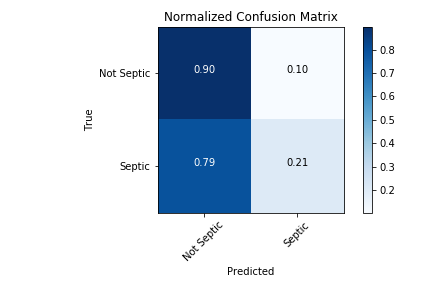
\includegraphics[scale=0.6]{bayesConfusion}
\caption{Naive Bayes Model Confusion Matrix}\label{fig:confusion}
\end{figure}

For the initial analysis we included all features recorded at least 4 hours 
before the sepsis event.  However, in our next iteration, we will construct gradient boosting models on increasing
time intervals as described previously. 

\section{Conclusion}
In this work, we have built a benchmark designed to facilitate construction of models for predicting sepsis
based on the MIMIC III database.  The benchmark provides features adjusted as needed for consistent units, with obvious coding
errors removed, following the previous work of Johnson et al.\cite{johnson2017}  These datasets can be used as we have done 
to compute SOFA scores for labeling patients, or users may determine their own labeling criteria.  The benchmark includes
clinical features that are available in a wide variety of medical settings, in order to encourage modeling approaches that can be
deployed in settings without access to the most advanced technology.

We have also developed a modeling approach for predicing onset of sepsis, using a cohort of patients aged 18 and above
from our benchmark.  We labeled patients as septic based on a clinically-validated approach using SOFA scores.\cite{jones2009}
This approach consisted of determining ``sepsis windows'' bounded by initial suspicion of infection and end of the last
ICU stay.  We then compared hourly SOFA scores for each patient to the SOFA score at the beginning of the corresponding
window.  We identified onset of sepsis as the first hour at which a patient's SOFA score increased by 2 or more
points.  This yielded a 23\% incidence of sepsis, which is consistent with ICU incidence during the
timeframe corresponding to the MIMIC III database.\cite{nee2006}  Using a Naive Bayes approach for initial investigation, 
we constructed a model that achieved an accuracy of 0.808 on a test fraction of 20\%.  While it is not good at 
identifying septic patients, it serves as a useful ``first draft'' of our modeling pipeline.  We are continuing to work on the 
gradient boosting model pipeline.  This will train models on successive windows of data and enable prediction of sepsis at
4-hour increments during a hospital stay.  We will again evaluate using an 80-20 split for training and testing.  In addition
to evaluating based on metrics such as accuracy and AUC, we will also specifically evaluate the false alarm rate in order
to estimate ``alert fatigue'' in the clinical setting.
  
\makeatletter
\renewcommand{\@biblabel}[1]{\hfill #1.}
\makeatother


\bibliographystyle{unsrt}
\begin{thebibliography}{1}
\setlength\itemsep{-0.1em}

\bibitem{desautels2016}
	T. Desautels, J. Calvert, J. Hoffman, M. Jay, Y. Kerem, L. Shieh,
	D. Shimabukuro, U. Chettipally, M. D. Feldman, C. Barton, D. J. Wales,
	and R. Das. Prediction of sepsis in the intensive care unit with minimal
	electronic health record data: A machine learning approach. 
	{\it JMIR Med Inform}, 4(3):e28, 30 Sept. 2016.

%\bibitem{harutyunyan2017}
%	H. Harutyunyan, H. Khachatrian, D. C. Kale, and A. Galstyan. Multitask
%	learning and benchmarking with clinical time series data. 
%	{\it arXiv preprint arXiv:1703.07771}, 22 Mar. 2017.	

\bibitem{henry2015}
	K. E. Henry, D. N. Hager, P. J. Pronovost, and S. Saria. A targeted
	real-time early warning score (trewscore) for septic shock. 
	{\it Science translational medicine}, 7(299):299ra122--299ra122, 2015.

\bibitem{coopersmith2018}
        Coopersmith, C. M., De Backer, D., Deutschman, C. S., Ferrer, R., Lat, I., Machado, F. R., 
        ... and Evans, L. E. Surviving sepsis campaign: research priorities for sepsis and septic shock. 
        {\it Intensive care medicine}, 44(9), 1400--1426. Sep. 2018.

\bibitem{futoma2017}
        Futoma, J., Hariharan, S., and Heller, K. Learning to detect sepsis with a multitask gaussian 
        process RNN classifier. {\it arXiv preprint arXiv:1706.04152}, 13 Jun. 2017.

\bibitem{horng2017}
        Horng, S., Sontag, D. A., Halpern, Y., Jernite, Y., Shapiro, N. I., and Nathanson, L. A. 
        Creating an automated trigger for sepsis clinical decision support at emergency department 
        triage using machine learning. {\it PloS one}, 12(4), e0174708. 6 Apr. 2017.

\bibitem{kam2017}
        Kam, H. J., and Kim, H. Y. Learning representations for the early detection of sepsis with deep neural 
        networks. {\it Computers in biology and medicine}, 89, 248--255. 1 Oct. 2017.

\bibitem{manaktala2016}
        Manaktala, S., and Claypool, S. R. Evaluating the impact of a computerized surveillance algorithm and 
        decision support system on sepsis mortality. {\it Journ Am Med Inform Assoc}, 
        24(1), 88--95. 25 May. 2016.

\bibitem{mayhew2018}
        Mayhew, M. B., Petersen, B. K., Sales, A. P., Greene, J. D., Liu, V. X., and Wasson, T. S. 
        Flexible, cluster-based analysis of the electronic medical record of sepsis with 
        composite mixture models. {\it Journ Biomed Inform}, 78, 33--42. 1 Feb. 2018.

\bibitem{mccoy2017}
        McCoy, A., and Das, R. Reducing patient mortality, length of stay and readmissions through machine 
        learning-based sepsis prediction in the emergency department, intensive care unit and hospital 
        floor units. {\it BMJ Open Qual}, 6(2), e000158. 1 Oct. 2017.

\bibitem{rothman2017}
        Rothman, M., Levy, M., Dellinger, R. P., Jones, S. L., Fogerty, R. L., Voelker, K. G., ... and Beals IV, J. 
        Sepsis as 2 problems: Identifying sepsis at admission and predicting onset in the hospital using an electronic 
        medical record-based acuity score. {\it Journ Crit Care}, 38, 237--244. 1 Apr. 2017.

%\bibitem{taneja2017}
%        Taneja, I., Reddy, B., Damhorst, G., Zhao, S. D., Hassan, U., Price, Z., ... and Winter, J. 
%        Combining biomarkers with EMR data to identify patients in different phases of sepsis. 
%        {\it Scientific Reports}, 7(1), 10800. 7 Sep. 2017.

\bibitem{singer2016}
        Singer, M., Deutschman, C. S., Seymour, C. W., Shankar-Hari, M., Annane, D., Bauer, M., ... and
        Angus, D. C. (2016). The third international consensus definitions for sepsis and septic shock (Sepsis-3). 
        {\it JAMA}, 315(8), 801--810. 23 Feb. 2016.

\bibitem{guirgis2017}
        Guirgis, F. W., Jones, L., Esma, R., Weiss, A., McCurdy, K., Ferreira, J., ... and Gerdik, C. 
        Managing sepsis: electronic recognition, rapid response teams, and standardized care save lives. 
        {\it Journ Crit Care}, 40, 296--302. 1 Aug. 2017.

\bibitem{liu2017}
        Liu, V. X., Fielding-Singh, V., Greene, J. D., Baker, J. M., Iwashyna, T. J., Bhattacharya, J., and 
        Escobar, G. J. The timing of early antibiotics and hospital mortality in sepsis. 
        {\it Am Journ Resp Crit Care Med}, 196(7), 856--863. 1 Oct. 2017.

\bibitem{macdonald2017}
        Macdonald, S. P., Williams, J. M., Shetty, A., Bellomo, R., Finfer, S., Shapiro, N., and Keijzers, G. 
        Sepsis in the emergency department--- Part 1: definitions and outcomes. 
        {\it Emergency Medicine Australasia}, 29(6), 619--625. Dec. 2017.

\bibitem{pollard2016}
        Pollard, T. J. and Johnson, A. E. W. 
        The MIMIC-III Clinical Database. http://dx.doi.org/10.13026/C2XW26 (2016).

\bibitem{jones2009}
        Jones, A. E., Trzeciak, S., and Kline, J. A. (2009). 
        The Sequential Organ Failure Assessment score for predicting outcome in patients with 
        severe sepsis and evidence of hypoperfusion at the time of emergency department presentation. 
        Crit. care med., 37(5), 1649.

\bibitem{johnson2017}
        Johnson, A. E. W., Stone D. J., Celi L. A., Pollardand T. J. 
        The MIMIC Code Repository: enabling reproducibility in critical care research.
        Journ Am. Med. Inform. Assoc. (2017): ocx084.

\bibitem{nee2006}
         Nee, P. A. (2006). 
         Critical care in the emergency department: severe sepsis and septic shock. 
         Emergency medicine journal, 23(9), 713-717.
\end{thebibliography}



\end{document}

